%%%%%%%%%%%%%%%%%%%%%%%%%%%%%%%%%%%%%%%%%
% University Assignment Title Page 
% LaTeX Template
% Version 1.0 (27/12/12)
%
% This template has been downloaded from:
% http://www.LaTeXTemplates.com
%
% Original author:
% WikiBooks (http://en.wikibooks.org/wiki/LaTeX/Title_Creation)
%
% License:
% CC BY-NC-SA 3.0 (http://creativecommons.org/licenses/by-nc-sa/3.0/)
% 
% Instructions for using this template:
% This title page is capable of being compiled as is. This is not useful for 
% including it in another document. To do this, you have two options: 
%
% 1) Copy/paste everything between \begin{document} and \end{document} 
% starting at \begin{titlepage} and paste this into another LaTeX file where you 
% want your title page.
% OR
% 2) Remove everything outside the \begin{titlepage} and \end{titlepage} and 
% move this file to the same directory as the LaTeX file you wish to add it to. 
% Then add \input{./title_page_1.tex} to your LaTeX file where you want your
% title page.
%
%%%%%%%%%%%%%%%%%%%%%%%%%%%%%%%%%%%%%%%%%
%\title{Title page with logo}
%----------------------------------------------------------------------------------------
%	PACKAGES AND OTHER DOCUMENT CONFIGURATIONS
%----------------------------------------------------------------------------------------

\documentclass[12pt]{article}
\usepackage[margin=1in]{geometry}
\usepackage[english]{babel}
\usepackage{url}
\usepackage[utf8x]{inputenc}
\usepackage{amsmath}
\usepackage{graphicx}
\usepackage[colorinlistoftodos]{todonotes}
\usepackage[sort, numbers]{natbib}
\usepackage[font=small,labelfont=bf]{caption}
\usepackage[hidelinks]{hyperref}
\usepackage{enumitem}
\setlist[itemize]{noitemsep, topsep=0pt}
\graphicspath{img/}


\usepackage{caption}
\DeclareCaptionFormat{citation}{%
   \ifx\captioncitation\relax\relax\else
     \captioncitation\par
   \fi
   #1#2#3\par}
\newcommand*\setcaptioncitation[1]{\def\captioncitation{\textit{Image source:}~#1}}
\let\captioncitation\relax
\captionsetup{format=citation,justification=centering}

\begin{document}

\begin{titlepage}

\newcommand{\HRule}{\rule{\linewidth}{0.5mm}} % Defines a new command for the horizontal lines, change thickness here

\center % Center everything on the page
 
%----------------------------------------------------------------------------------------
%	HEADING SECTIONS
%----------------------------------------------------------------------------------------

\textsc{\LARGE Ukrainian Catholic University}\\[1cm] % Name of your university/college
\textsc{\Large Applied Sciences Faculty}\\[0.5cm] % Major heading such as course name
\textsc{\large Data Science Master Programme}\\[0.5cm] % Minor heading such as course title

%----------------------------------------------------------------------------------------
%	TITLE SECTION
%----------------------------------------------------------------------------------------

\HRule \\[0.4cm]
{ \huge \bfseries Abstractive text summarization with Recurrent Neural
	Networks}\\[25pt]
{\Large \bfseries Machine Learning project report}\\[0.4cm] % Title of your document
\HRule \\[0.8cm]
 
%----------------------------------------------------------------------------------------
%	AUTHOR SECTION
%----------------------------------------------------------------------------------------


% If you don't want a supervisor, uncomment the two lines below and remove the section above
\Large \emph{Authors:}\\
Hanna \textsc{Pylieva}\\Yuriy \textsc{Mykhalchuk}\\Irynei \textsc{Baran}\\[0.5cm] % Your name

%----------------------------------------------------------------------------------------
%	DATE SECTION
%----------------------------------------------------------------------------------------

{\large \today}\\[2cm] % Date, change the \today to a set date if you want to be precise

%----------------------------------------------------------------------------------------
%	LOGO SECTION
%----------------------------------------------------------------------------------------


\includegraphics[height=4cm]{img/UCU-Apps.png}\\[1cm] % Include a department/university logo - this will require the graphicx package
 
%----------------------------------------------------------------------------------------

\vfill % Fill the rest of the page with whitespace

\end{titlepage}


\begin{abstract}
In this work, we describe the process of resolving abstactive text summarization task as sequence-to-sequence problem. We trained encoder-decoder LSTM-based model with attention mechanism for generating captions of news articles. 
\end{abstract}

\section{Introduction}

In the modern Internet age, textual data is ever increasing. According to this each Internet user will highly benefit from condensing data while preserving the information and meaning. This idea is a driver of growing interest among the research community for developing new approaches to automatically summarize the text. Automatic text summarization system generates a short summary that captures the main ideas
of an input text. Since the advent of text summarization in 1950s, researchers have been trying to improve techniques for generating machine summaries which are not worse than human made summaries \cite{text_sum_survey}.
  
There are two prominent types of summarization algorithms.

\begin{itemize}
\setlength\itemsep{0.5em}

	\item Extractive summarization copies parts of the source text through some measure of importance and then combines those part/sentences together to render a summary. Importance of sentence is based on linguistic and statistical features.

	\item Abstractive summarization generates new phrases, possibly rephrasing or using words that were not in the original text. Naturally abstractive approaches are harder as it involves robust natural language processing. For perfect abstractive summary, the model has to first understand the document and then express that understanding in succinct form possibly using new words and phrases.  Abstractive summarization has complex capabilities like generalization, paraphrasing and incorporating  real-world knowledge \cite{abstractive_text_summarization}.
\end{itemize}

Majority of the work has traditionally focused on extractive approaches due to the easy of defining hard-coded rules to select important sentences than generate new ones. Also, it promises grammatically correct and coherent summary. But they often don’t summarize long and complex texts well as they are very restrictive.


Abstractive methods, on the other hand, provide highly powerful and promising results. That is why in this project we implemented an algorithm for abstractive text summarization to build solid understanding of this approach and discover how it can be improved.


\section{Model}
\subsection{Background}
Models for abstractive text summarization fall under a larger deep learning category called
sequence-to-sequence models, which map from an input sequence to a target sequence. This approach is illustrated on Figure~\ref{fig:seq-to-seq}. It was initially used for Neural Machine Translation as described in \cite{attention_based_NMT}. 


\begin{figure}[ht]
	\centering
	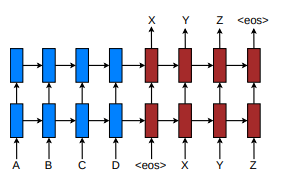
\includegraphics[width=0.5\textwidth]{img/seq-to-seq.png}
	\setcaptioncitation{\cite{attention_based_NMT}}
	\caption{\label{fig:seq-to-seq}The model reads an input sentence “A B C D” and produces “X Y Z” one word by word as output sentence. The model stops making predictions after outputting the $<$eos$>$ token.  }
\end{figure}


An effective and standard approach to build sequence-to-sequence models is using Encoder-Decoder architecture that act as an encoder and a decoder pair. The encoder reads the entire input sequence and encodes it into an internal representation, often a fixed-length vector called the context vector. The decoder reads the encoded input sequence and generates the output sequence. Both the encoder and the decoder submodels are trained jointly, i.e. at the same time.

Naturally we need the input and output to be of variable length. This can not be reached with ordinary Deep Neural Networks (DNNs) which require that the dimensionality of the inputs and outputs is known and fixed. 

The Recurrent Neural Networks (RNNs) are generalization of feedforward neural networks to sequences. Given a sequence of inputs $(x_1, ..., x_T)$, a standard RNN computes a
sequence of outputs $(y_1, ..., y_T)$ by iterating the following equation \cite{seq2seq_with_NN} :

\begin{equation}
\begin{array}{l}
	h_t = f(W^{hx}x_t + W^{hh}h_{t-1}) \\
	y_t = W^{yh}h_t
\end{array}
\end{equation}
where 
$f$ - activation function,
$x_{t}$ - input vector, 
$h_{t}$ - hidden layer vector,
$y_{t}$ - output vector,
$W$ - weight matrix
 
 
An RNN can map sequences to sequences provided that the alignment between the inputs and the outputs is known ahead. In other words RNN needs a defined one-to-one correspondence between a sequence of inputs and sequence of outputs which can be understood better from RNN unfolded representation on Figure~\ref{fig:RNN}.

\begin{figure}[ht]
	\centering
	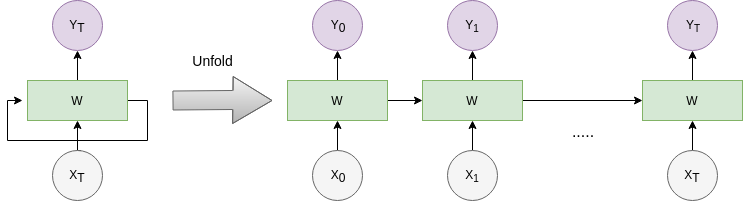
\includegraphics[width=0.6\textwidth]{img/RNN.png}
	\setcaptioncitation{Created by author}
	\caption{\label{fig:RNN}Recurrent Neural Network}
\end{figure}
 
However, it is not clear how to apply an RNN to problems whose input and the output sequences have different lengths with complicated and non-monotonic relationships.

The simplest strategy for general sequence learning is to map the input sequence to a fixed-sized
vector using one RNN, and then to map that vector to the target sequence with another RNN (the
approach is represented in \cite{baseline_NMT}). Since the RNN is provided with all the relevant information this will work. Whereas the need to store information over extended time interval will lead to difficulties with training RNN (vanishing/ exploding gradient problem explained in \cite{LSTM_baseline}).
Here Long Short-Term Memory (LSTM) layers will come in handy as they are known to learn problems with long range temporal dependencies and will succeed in this setting.

\subsubsection{LSTM}

The goal of LSTM is to estimate the conditional probability of output sequence by input sequence $p(y_1, ..., y_{T′}|x_1, ..., x_T )$ when lengths of those sequences are possibly different ($T' \neq T$). 
An LSTM computes this conditional probability by first obtaining the fixed dimensional
representation $v$ of the input sequence $(x_1, ..., x_T)$ given by the last hidden state of the LSTM, and then computing the probability of $y_1, ..., y_{T′}$ with a standard LSTM-LM
\footnote{Language Model (LM) is a probability distribution over sequences of words. LSTM-LM is an algorithm of using an LSTM (and softmax function) to predict the next word given your previous words.} 
formulation whose initial hidden state is set to the representation $v$ of  $x_1, ..., x_T$:

$$p(y_1, ..., y_{T′}|x_1, ..., x_T ) = \prod_{t=1}^{T'} p(y_t|v, y_1, ..., y_{t-1}) $$


In this equation, each $p(y_t|v, y_1, ..., y_{t-1})$ distribution is represented with a softmax over all the
words in the vocabulary \cite{seq2seq_with_NN}.

Taking into consideration all above and having processed prominent researches on abstractive summarization topic we've built an encoder-decoder recurrent neural network with LSTM units and attention mechanism to generate headlines from the text of news articles. We took the model described in \cite{model-baseline-article} as baseline, but performed some modifications according to available software restrictions. We used the next repository as a reference point of how to build the whole process \cite{reference-repository}.

\subsection{Overview}
In our model encoder and decoder get more precise descriptions.

\subsubsection{Encoder}
The input of encoder consists of article's text of restricted size followed by an end-of-sequence symbol ($EOS$, in code we used '$<eos>$') followed by header. Each word of input is first passed through an embedding layer which transforms it into a distributed representation.
% So now each word has a corresponding vector $w \in R^d$.
We run the stacked LSTMs over the sequence of vectors and store the last hidden state $v \in R^H$ - this is a fixed-size encoder representation, which will be used by decoder to generate the target sequence word by word.   

\subsubsection{Decoder}
On each decoding step we feed $v$ as hidden state and the word generated on previous step (EOS symbol on the first step) into decoder as input.
% The LSTM computes next hidden state of decoder $h_0 \in R^h$. 
Then a function $g: R^H \rightarrow R^V$ is applied so that $s_t := g(s_{t-1}, [v, y_{t-1}]) \in R^V$ is a vector of the same size as vocabulary ($s_0 := g([v, <eos>]$). Then we predict next word $y_t$ in output sequence by applying softmax to $s_j$. The softmax function results in a vector of likelihood for each word in the vocabulary to be the next in the sequence. 

The task of decoder is to find the most likely output sequence for the input received and processed by encoder. Due to big vocabulary size the search problem through all the possible output sequences based on their likelihood is exponential in length of the output sequence and is NP-complete. That is why it is common to use approximate methods. We used beam search and were keeping in memory 10 best hypotheses (output sequences) to eventually opt for the best combination of words (Figure~\ref{fig:encoder-decoder-lstm}). 

\begin{figure}[h]
\centering
	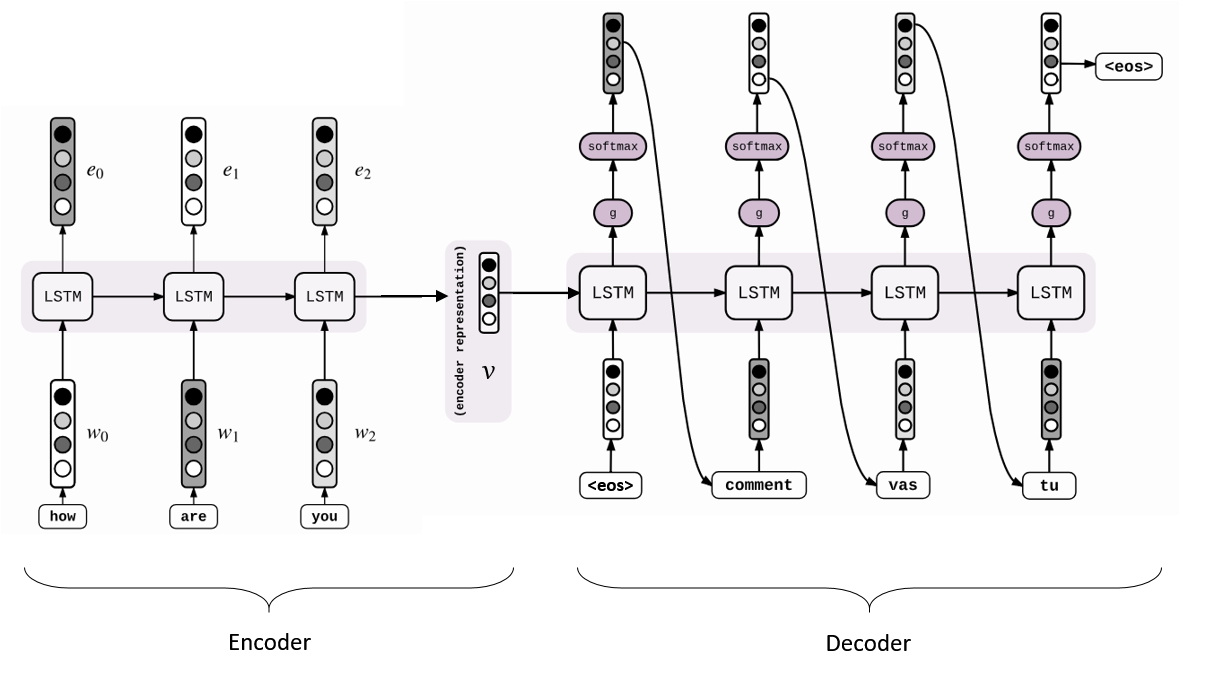
\includegraphics[width=0.8\textwidth]{img/seq2seq-detailed.png}
	\setcaptioncitation{Created by author, inspired by \cite{seq2seq-explanation} }
	\caption{\label{fig:encoder-decoder-lstm}LSTM-based sequence to sequence model on example of NMT. Note: $v$ is actually fed on input of decoder on each step to prevent neural network from "forgetting" about it till the end of output sequence. }
\end{figure}


The described process corresponds to testing phase. On training phase instead of feeding in as input of new generative step the freshly generated word, the expected word from the actual headline is fed in. This leads to a disconnect between training and testing. To overcome this disconnect, during training we randomly feed in a generated word, instead of the expected word, as suggested in \cite{scheduled_sampling}. Specifically, we do this for 10\% of cases. This approach is called "teacher forcing".

%\begin{equation}
%\begin{array}{l}
%	h_0 = LSTM(v, [w_{eos}, c_t]) \\
%	s_0 = g(h_0) \\
%	p_0 = softmax(s_0)\\
%	i_0 = argmax(p_0)\\
%	
%	t = 1\\
%	while \; w_{i{t-1}} \neq w_{eos}:\\
%\quad		h_t = LSTM(e, [w_{i{t-1}}, c_t])\\
%\quad		s_t = g(h_t)\\
%\quad		p_t = softmax(s_t)\\
%\quad		i_t = argmax(p_t)\\
%\quad		t += 1	\\
%\end{array}
%\end{equation}


\subsubsection{Attention} \label{attention}
In the vanilla encoder-decoder architecture encoder reads the input sequence of words and compresses all the information into a fixed-length vector of hidden states. This can lead to significant information loss and inadequate summarization in case of long input sequences, because hundreds of words will be represented by several of them. Attention mechanism is aimed to fix this problem. It speeds up the learning and lifts the skill of the model on sequence to sequence prediction problems. 

The attention mechanism is used when outputting each word in the decoder (Figure~\ref{fig:attention}). For each output word the attention mechanism computes a weight over each of the input words that determines how much attention should be paid to that input word. The weights sum up to 1, and are used to compute a weighted average of the last hidden layers generated after processing
each of the input words. This weighted average, referred to as the context, is then fed into the softmax layer along with the last hidden layer from the current step of the decoding.
%With attention mechanism the decoder relies not only on a single hidden state generated by encoder, but has information about hidden states $\{h_i\}$ generated by encoder on each time stamp.  

\begin{figure}[h]
\centering
	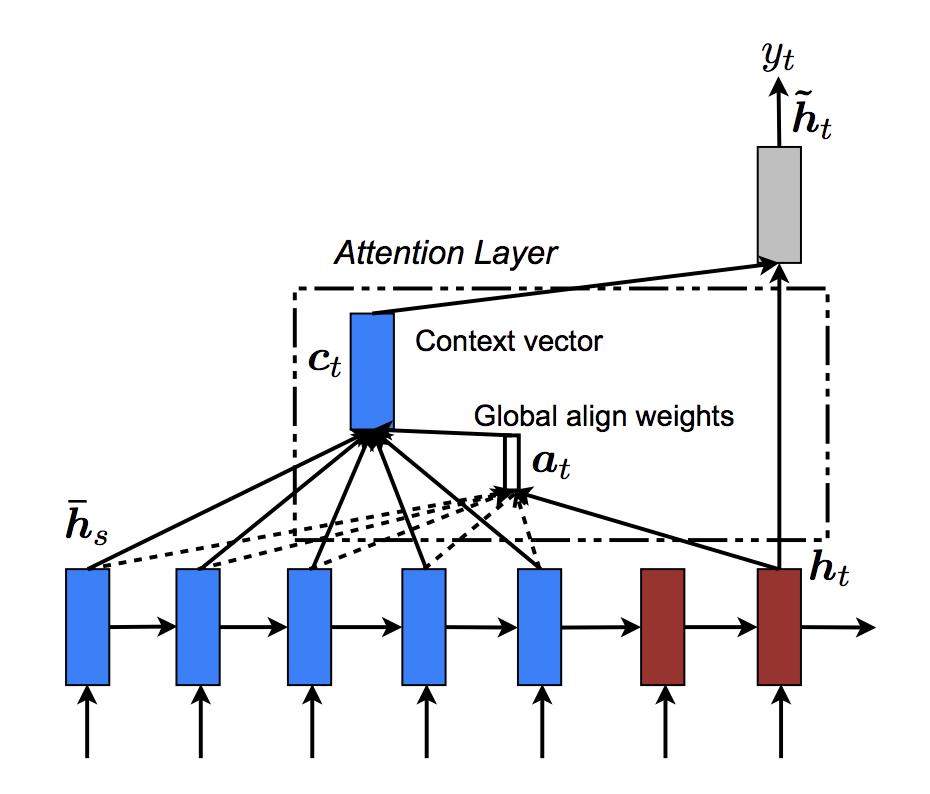
\includegraphics[width=0.5\textwidth]{img/seq2seq-with-attention.png}
	\setcaptioncitation{\cite{attention_based_NMT}}
	\caption{\label{fig:attention}Global Attention in an Encoder-Decoder Recurrent Neural Network}
\end{figure}


\subsubsection{Training details}

We used Google Colaboratory to process data, train and text model. Colaboratory is a research tool for machine learning education and research. It is a Jupyter notebook environment that requires no setup to use. 
Colaboratory is free and allows a group of users edit one Jupyter notebook simultaneously. Google Colab has 12Gb free RAM and allows using one Tesla K80 GPU with Keras and Tensorflow.

Our solution is implemented on Python3, the model is built on Keras with Tensorflow backend. 

According to RAM limitation and politics of Google Colaboratory to switch off processes which run for more than 12 hours (to prevent cryptocurrency mining on the tool), we had issues during training as it was insufficient for our purposes. Mostly the models like the one described are run during 3-8 days in case of one GPU as they use a big input dataset and deep LSTMs. As we had only 1 GPU, the maximum model characteristics which allowed us run at least one epoch in a time without fails were the following:

\begin{itemize}
\item Maximum length of description (in words): 25 . Description is an article. So we took only 25 first words from each article. 
\item Maximum length of header (in words): 25. Header is a caption of article.
\item Number of RNN (LSTM) layers: 3
\item Dimensionality of output from RNN: 128
\item Batch-size: 64
\item Vocabulary size: 40000
\item Size of input dataset(number of articles): 100000 (10 times less than the size of dowloaded dataset from the source)
\item Learning rate: started with 0.01, then changed to 0.0001
\end{itemize}

As we experienced "Runtime died" frequently, our model saves weights after each epoch. Each epoch took up to 1 hour. The best loss we reached on validation set was 7.8181 (started from 20.0). We managed to run our model for at most 8 epochs without failures.

\section{Dataset}
\subsection{Overview}
We used \href{http://research.signalmedia.co/newsir16/signal-dataset.html}{The Signal Media One-Million News Articles Dataset}. It contains 1 million articles that are mainly English, but they also include non-English and multi-lingual articles. Sources of these articles include major ones, such as Reuters, in addition to local news sources and blogs.

The file is in JSONL format, where each line is a JSON object representing an article. Each article has the following fields:

\begin{itemize}
%\setlength\itemsep{-0.5em}
\item id: a unique identifier for the article
\item title: the title of the article
\item content: the textual content of the article (may occasionally contain HTML and JavaScript content)
\item source: the name of the article source (e.g. Reuters)
\item published: the publication date of the article
\item media-type: either "News" or "Blog"
\end{itemize}  

We extracted only "content" and "title" fields, then serialized then into ,pkl to make reads more convenient.

\subsection{Preprocessing}
During data preprocessing we did the following:

\begin{enumerate}[noitemsep]
%\setlength\itemsep{-0.5em}
\item Converted the original file into standard JSON format and left only "content" and "title" fields.
\item Left only two sentences in descriptions
\item Tokenize data using nltk’s Punkt tokenizer
\item Got vocabulary and words counts of all words in dataset
\item Indexed all words in vocabulary 
\item Created mappings from words to indexes and vice versa
\item Read GloVe embeddings (with dimetionality of vectors 100), set embeddings for lowercased words the same as for original ones if the lowercased version has no embedding
\item Initialized embedding matrix for 40k of the most popular words uniformly at random
\item For each word among those 40k which has embedding in Glove set this embedding to an appropriate row in the embedding matrix 
\item Found embeddings for all words which are not the most popular, but are present in Glove
\item For words from the previous step found the nearest embedding of a word from most popular words and assigned to this non popular word (this helped to find embeddings for 187k additional words)
\item Replaced words with their indices in headlines and descriptions
\item Serialized the next:
	\begin{itemize}
		\item indexed headlines
		\item indexed descriptions
		\item embedding for the most popular words from vocabulary
 		\item mappings between words from vocabulary and their indices and vice versa
 		\item mappings between words from vocabulary and words from Glove
	\end{itemize}
 	
\end{enumerate}


\section{Results Analysis}

The examples of meaningful headers generated by our model are represented in 
Table ~\ref{tab:results-table}.

There are a lot of nonsense headers which our model generates, so there is obviously a big area for improvement of our model. Training on physical GPU or more reliable Cloud than Google Colaboratory for more epochs should improve the results significantly.

What we have mentioned for now is that our model likes to put out-of-vocabulary words in caption. For example, one of generated headers for the third example in table was "Business Cash Lockscreen\^{} the : Lockscreen\^{} and ( to and Lockscreen\^{} ) , 2015 Nikhil after key issued price Agency". Such behavior is caused by high attention on such words. Also model does not recognize a multy-word entities, i.e. in the same example we have "Echo Notification Lockscreen" entity, but in headers we mostly observed only "Lockscreen" appears as "echo" and "notification" are known words.

What is important to note, our model doesn't rephrase the ground truth headline, but generates its own.

Our code for data preprocessing, model testing and training can be found \href{https://github.com/mykhaly/text_summarization_using_LSTM}{[here]}.

\begin{center}
\begin{table}[!htb]
\centering
\caption{Example predictions}
\label{tab:results-table}
\begin{tabular}{|l|l|l|}
\hline
\textbf{Text} & \textbf{Actual Headline} & \textbf{Predicted Headline} \\ \hline

\begin{minipage}[t]{0.4\columnwidth}%
Sydney-based strategic integrated communications agency, Zadro, has moved to the next level; due to the business expansion, they are commencing a new chapter in their growth by relocating to a bigger, better and brighter office space in Surry Hills. Felicity Zadro, Managing Director, Zadro, says the move is indicative of the way the agency has flourished since its inception eight years ago.             
\end{minipage}
 & 
\begin{minipage}[t]{0.3\columnwidth}%
 Integrated communications agency, Zadro, moves to the next level. 
\end{minipage}
 & 
\begin{minipage}[t]{0.3\columnwidth}% 
 Launches in Sydney-based Zadro. 
\end{minipage}  \\ \hline

\begin{minipage}[t]{0.4\columnwidth}%
Shares of Toronto-Dominion Bank (NYSE: TD) have been given an average recommendation of Buy by the eleven research firms that are currently covering the firm, Market Beat Ratings reports. One equities research analyst has rated the stock with a sell rating, three have assigned a hold rating and six have given a buy rating to the company.           
\end{minipage}
 & 
\begin{minipage}[t]{0.3\columnwidth}%
Toronto-Dominion Bank Receives \$56.75 Average Target Price from Analysts (NYSE: TD) 
\end{minipage}
 & 
\begin{minipage}[t]{0.3\columnwidth}% 
Report of Products Market Toronto-Dominion. 
\end{minipage}  \\ \hline

\begin{minipage}[t]{0.4\columnwidth}%
Microsoft has acquired Double Labs, an Android app startup which develops the popular Echo Notification Lockscreen for Android devices. This app had received between 1 million and 5 million downloads so far in Play Store.          
\end{minipage}
 & 
\begin{minipage}[t]{0.3\columnwidth}%
Microsoft Acquires Popular Android App Echo Notification Lockscreen
\end{minipage}
 & 
\begin{minipage}[t]{0.3\columnwidth}% 
Lockscreen Management Announces
\end{minipage}  \\ \hline

\end{tabular}
\end{table}
\end{center}



\pagebreak

\begin{thebibliography}{9}
	
	\bibitem{text_sum_survey}
	Gambhir, M. and Gupta, V. \textit{Recent automatic text summarization techniques: a survey}. Artificial Intelligence Review, 47(1):1-66, 2017.
	
	\bibitem{abstractive_text_summarization}
	Singhal,S. and Bhattacharya, A. \textit{Abstractive Text Summarization}. Department of Computer Science IIT Kanpur, 2017.
	
	\bibitem{attention_based_NMT}
	Minh Thang Luong; Hieu Pham; Christopher D. Manning. \textit{Effective Approaches to Attention-based Neural Machine Translation}. CoRR, abs/1508.04025, 2015. \url{http://arxiv.org/abs/1508.04025}
	
	\bibitem{baseline_NMT}
	Bahdanau,D.; Cho,K.; Bengio Y. \textit{Neural machine translation by jointly learning to align and translate}. CoRR, abs/1409.0473, 2014. \url{ http://arxiv.org/abs/1409.0473}.
	
		
	\bibitem{LSTM_baseline}	
	S. Hochreiter and J. Schmidhuber. \textit{Long short-term memory}. Neural Computation, 1997.
	
	\bibitem{seq2seq_with_NN}
	Ilya Sutskever, Oriol Vinyals, Quoc V. Le \textit{Sequence to Sequence Learning with Neural Networks}. CoRR, abs/1409.3215, 2014. \url{http://arxiv.org/abs/1409.3215}

		 
	\bibitem{model-baseline-article}
	Lopyrev, K.\textit{Generating News Headlines with Recurrent Neural 	Networks}. CoRR, abs/1512.01712, 2015.
	
	
	\bibitem{reference-repository}
	 \url{https://github.com/udibr/headlines}
	 
	 \bibitem{seq2seq-explanation}
	 \url{https://guillaumegenthial.github.io/sequence-to-sequence.html}
	
	\bibitem{scheduled_sampling}
	Samy Bengio, Oriol Vinyals, Navdeep Jaitly, and Noam Shazeer. \textit{Scheduled sampling for sequence
prediction with recurrent neural networks}. CoRR, abs/1506.03099, 2015. \url{http://arxiv.org/abs/1506.03099}

	\bibitem{bleu}
Kishore Papineni, Salim Roukos, Todd Ward, and Wei-Jing Zhu.\textit{BLEU: A method for automatic evaluation of machine translation}. In Proceedings of the 40th Annual Meeting on Association for Computational Linguistics, ACL ’02: 311–318, Stroudsburg, 2002. 
	
%	\bibitem{deep_learning_basic}
%	Ian Goodfellow, Yoshua Bengio, Aaron Courville \textit{Deep Learning}. MIT Press. 2016. \url{http://www.deeplearningbook.org/}
	
%	\bibitem{bishop}
%	Bishop, Christopher M.	\textit{Pattern Recognition and Machine Learning}. %Springer, Cambridge, U.K., 2006.

\end{thebibliography}


\end{document}